\documentclass[10pt, a4paper]{proc}
\usepackage[utf8]{inputenc}
\usepackage{setspace}
\usepackage{ragged2e}
\usepackage{fancyhdr}
\usepackage{graphicx}
\usepackage{titlesec}
\usepackage[T2A]{fontenc}
\usepackage{tikz}  
\usepackage{amsmath}
\usepackage{tempora}
\usepackage{enumitem}
\usetikzlibrary{graphs, positioning, arrows.meta}
\usepackage[left=2.5cm,right=2.5cm,
    top=2.5cm,bottom=2.5cm]{geometry}
\justifying
\fancyhf{} 
\renewcommand{\headrulewidth}{0pt} 
\cfoot{\vskip -1.5cm \thepage}
\pagestyle{fancy}
\linespread{0.85}
\setlength{\columnsep}{0.5cm}
\setcounter{page}{165}
\renewcommand{\thesection}{\Roman{section}}
\titleformat{\section}{\large\centering\sc}{\thesection. }{0cm}{}[]

\title{
 \begin{spacing}{1}
 
  {\textbf{\Huge{Neuro-semantic Industrial Control}}}
 \end{spacing}
}

\author{
 \linespread{1.3} Dzmitry Ivaniuk\\\textit{JSC “Savushkin}\\Product”Brest, Republic of Belarus\\Email:Ivaniuk.Dzmitry@savushkin.com\\
 }

\date{September 2024}

\begin{document}

\maketitle

\fontsize{9}{13.7}\selectfont{
\textbf{\textit{Abstract}—This article provides a review of the current
situation of ontology use in industrial control with help
of OSTIS Technology, examines in more detail the issues
of combining together classical approach (standards in the
field of Industry 4.0, such as ISA-88, ISA-95 and ISA
5.1) and intelligent technologies (neuro-control as part of
Artificial Intelligence, AI) between robots (robotic systems)
and humans.}  \par
\textbf{\textit{Keywords}—Semantic analysis, OSTIS technology, Wolfram Mathematica, Wolfram Knowledgebase, Entity, temporal markers, Nevod }}

\fontsize{10}{13.7}\selectfont{  

 \section{\usefont{T2A}{Tempora-TLF}{m}{n}\normalsize{Introduction}}
 
This work expands on the ideas discussed in [1]–
[3] and includes descriptions of current issues and new
versions of suitable tools for developing and using standards in industry in relation to modern techniques (neurocontrol, semantic technologies).The connection with Industry 4.0 is taken into consideration, which is typically
characterized by its complexity and the need for comprehensive knowledge of models and techniques to achieve
an integrated solution [4].The arrival of Industry 4.0 has
made it necessary for technical systems to consider the
reliable and safe interaction of various intelligent systems
with each other [5]. By using Artificial Intelligence
decision making algorithms, process mapping in the
new Industry 5.0 scenario can be enhanced, particularly
by defining workflow checkpoints and identifying risks
related to production and product quality.
\par The important role is played by all participants in
the process: users — people (operators, masters, supervisors, etc.); devices — sensors and actuators (temperature sensors, pumps, valves, etc.); mechanized systems — conveyor systems, units; robotic systems —
hinged robots, delta robots, manipulators; and software
systems — SCADA, MES, ERP. Their interaction ensures the achievement of the goal, elimination and prevention of emergency situations. And important influence
have both quantitative indicators (number of operators,
devices, aggregates, control panels, etc.) and quality
(quality of devices, qualification of operators, quality of
software systems, etc.). Also important in management
systems is the speed of decision-making — making
changes quickly to meet plans. Each level is controlled
by its own algorithms — often the element may look like
a black box: input and output data are known, and the
inputs neural network outputs
Figure 1. Neural network as a black box
algorithm is hidden from the user. For instance, a neural
network can so be described (Fig. \ref{fig:M1}).

\begin{figure}
\quad\normalsize{
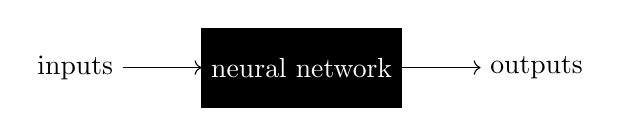
\begin{tikzpicture}[
squarednode/.style={rectangle, draw=white},
blacksquarednode/.style={rectangle, draw=black, fill=black, minimum height=1cm},
]

\node[squarednode]      (maintopic)                              {inputs};
\node[blacksquarednode]      (rightsquare)       [right=of maintopic] {\textcolor{white}{neural network}};
\node[squarednode]      (rightsquare2)       [right=of rightsquare] {outputs};
%Lines
%Lines
\draw[->] (maintopic.east) -- (rightsquare.west);
\draw[->] (rightsquare.east) -- (rightsquare2.west);
\end{tikzpicture}
\caption{Neural network as a black box
} \label{fig:M1}}
\end{figure}

\par But if you want to have some more subtle configuration, you have to go to the documentation and use
specific tools (for example, a change in the structure
of the neural network may involve additional training or
full new training on new reference data, which may also
be unavailable and will require additional creation or/or
adaptation of existing ones). The ontological description
provides a general description that can be understood by
all the participants. An integrated approach is needed
to create a fundamentally new generation of intelligent
computer systems and a corresponding technological
complex.
\par Standardization describes different aspects of each developed human activity and includes a system of concepts
(including terminology), a typology, and a model that
describes how to apply appropriate methods and means,
production sites, types and structures of project documents, accompanying activities, etc. With the existence
of standards, we can solve one of the key problems
related to any technology, particularly the rapidly developing computer information technology, \textbf{compatibility
problem} [6]. Compatibility can be considered in many
aspects, from the consistency of terminology in the
interactions of process participants to the consistency
of actions taken in the process of technology application. On the one hand, the problem with cohesion of
digital twin models lies in the fact that a large number
of disparate, unrelated and heterogeneous models are
required. On the other hand, connecting digital twins
in a single system [7] requires their interaction, and
awaits conceptual unification of this interaction. It also
require from Supervisory Control And Data Acquisition
(SCADA) systems a higher level of integration, scalability and technological modernity [8].
\par Despite advances in information technology, most
standards are now presented in the form of traditional
linear documents or Web resources containing a series of static pages connected by hyperlinks. This approach
to expressing standards has many serious drawbacks,
and ultimately the overhead costs of maintaining and
using standards actually outweigh the benefits of using
them [9].

\section{\usefont{T2A}{Tempora-TLF}{m}{n}\normalsize{Problems and state of art}}

An analysis of the work has made it possible to
formulate the most important and common problems
related to the development and application of modern
standards in various fields [9], [10]:

\begin{itemize}[noitemsep]
\normalsize{
  \item Above all, the complexity of maintaining the standards themselves due to the duplication of information, especially the complexity of changing terminology.
  \item Duplicate information in the documentation describing the standard.
  \item Standards Internationalization Issues — translating
a standard into multiple languages actually requires
supporting and coordinating independent versions of
the standard in different languages.
\item As a result, inconsistencies in the format of different
standards. As a result, automating the process of
developing and applying standards is complicated.
\item The inconvenience of using the standard, especially
the complexity of finding the information you need.
As a result, the complexity of studying standards.
\item The complexity of automating the verification that
an object or process complies with the requirements
of a particular standard.
\item etc.}
\end{itemize}

These problems are mainly related to the presentation
of standards. The most promising approach to solve these
problems is the transformation of each specific standard
into a knowledge base, which is based on a set of
ontologies corresponding to this standard [6], [9]–[12].
This approach allows us to significantly automate the development processes of the standard and its application.
\par As an example, consider the \textbf{ISA-88} [13] standard
(the basic standard for batch production). Although this
standard is widely used by American and European
companies and is actively implemented on the territory
of the Republic of Belarus, it has a number of drawbacks.
Essential ISA batch systems standards are:

\begin{itemize}[noitemsep]
\normalsize{
\item \textit{ANSI/ISA-88.00.01-2010}, Batch Control — Part 1:
Models and Terminology;
\item \textit{ISA-88.00.02-2001}, Batch Control — Part 2: Data
Structures and Guidelines for Languages;
\item \textit{ANSI/ISA-TR88.00.02-2015}, Machine and Unit
States: An implementation example of ANSI/ISA88.00.01;
\item \textit{ISA-88.00.03-2003}, Batch Control — Part 3: General and Site Recipe Models and Representation;
\item \textit{ISA-TR88.0.03-1996}, Possible Recipe Procedure
Presentation Formats;
\item \textit{ANSI/ISA-88.00.04-2006}, Batch Control — Part 4:
Batch Production Records;
\item \textit{ISA-TR88.95.01-2008}, Using ISA-88 and ISA-95
Together;
\item \textit{IEC 61512-1}, The European version approved in
1997, based on the older version \textit{ISA-88.01-1995};
\item \textit{GOST R IEC 61512-1-2016} — Russian version of
the standard, identical to \textit{IEC 61512-1}.}
\end{itemize}

 Another standard often used in the context of Industry
4.0 is \textbf{ISA-95} [14]. \textbf{ISA-95} is an industry standard for
describing high-level control systems. Its main purpose
is to simplify the development of such systems, abstract
from the hardware implementation and provide a single
interface to interact with the ERP and MES layers.
Consists of the following parts:

\begin{itemize}[noitemsep]
\normalsize{
\item \textit{ANSI/ISA-95.00.01-2010}, Enterprise-Control System Integration — Part 1: Models and Terminology;
\item \textit{ANSI/ISA-95.00.02-2018}, Enterprise-Control System Integration — Part 2: Objects and Attributes
for Enterprise-Control System Integration;
\item \textit{ANSI/ISA-95.00.03-2013}, Enterprise-Control System Integration — Part 3: Activity Models of Manufacturing Operations Management;
\item \textit{ANSI/ISA-95.00.04-2018}, Enterprise-Control System Integration — Part 4: Objects and Attributes for
Manufacturing Operations Management Integration;
\item \textit{ANSI/ISA-95.00.05-2018}, Enterprise-Control System Integration — Part 5: Business-to Manufacturing Transactions;
\item \textit{ANSI/ISA-95.00.06-2014}, Enterprise-Control System Integration — Part 6: Messaging Service
Model;
\item \textit{ANSI/ISA-95.00.07-2017}, Enterprise-Control System Integration — Part 7: Alias Service Model;
\item \textit{ANSI/ISA-95.00.08-2020}, Enterprise-Control System Integration — Part 8: Information Exchange
Profiles.}
\end{itemize}

 Models help define boundaries between business and
control systems. They help answer questions about which
functions can perform which tasks and what information
must be exchanged between applications. The ISA5 standards development committee is often referred to as the
ISA-5.1 standard among practitioners. However, the ISA5
committee, “Documentation of Measurement and Control
Instruments and Systems,” has a broader scope—namely
to develop standards, recommended practices, and technical reports for documenting and illustrating measurement
and control instruments and systems suitable for all
industries. ISA5 standards consist of the following:

\begin{itemize}[noitemsep]
\normalsize{
\item \textit{ANSI/ISA-5.1-2022}, Instrumentation Symbols and
Identification;
\item \textit{ISA-5.9 working group}, Controller Algorithms and
Performance;
\item \textit{ISA-5.4}, Instrument Loop Diagrams;
166
\item \textit{ISA-5.5-1985}, Graphic Symbols for Process Displays;
\item \textit{ISA-5.6}, Documentation for Control Software Applications;}
\end{itemize}

This standard is useful when a reference to equipment
is required in the chemical, petroleum, power generation,
air conditioning, metal refining, and many other industries. The standard enables anyone with a reasonable level
of plant knowledge to read flow charts to understand how
to measure and control a process without having to go
into the details of instrumentation or the knowledge of
an instrumentation expert.
 
 \section{\usefont{T2A}{Tempora-TLF}{m}{n}\normalsize{Neurocontrol}}

Neurocontrol is a relatively young field of research
that became independent in 1988. However, research
in this area began much earlier. One of the definitions
the science of "cybernetics" considers this as a general
theory control and interaction not only of machines, but
also also biological beings. Neurocontrol tries to achieve
this position through the construction of control systems
(decision-making systems), which can be trained during
operation, and thus improve its performance. In this case,
such systems use parallel mechanisms of information
processing, like the brain of living organisms [15].
\par For a long time the idea of building a perfect control
system - a universal controller that would look like a
«black box» from the outside was popular. It could be
used to control any system, with connections to sensors,
actuators, other controllers, and a special link to the
«efficiency module» — a system that determines the
management efficiency based on given criteria. The user
of such a control system would only set the desired result,
the further trained controller would manage himself,
perhaps following a complex strategy of achieving the
desired result in the future. It would also constantly
adjust its management based on the management object’s
response to achieve maximum efficiency. An outline of
such a system is given below (Fig. \ref{fig:M2}).

 \section{\usefont{T2A}{Tempora-TLF}{m}{n}\normalsize{Developed Neuro-PID controller}}

The overall structure of the self-tuning neuro-PID
controller is shown in Fig. \ref{fig:M3}, where the neural network
(NN) outputs are proportional (K), integral (TI ), and
differential (Td) components [16].
\par To control the Pasteurizer [16] PID is configured with
a multilayer perceptron (MLP, neuro-PID adjuster) with
the following structure: 20 input, 10 hidden and 3 output
neural elements; the function of activating the hidden
and output layers is sigmoid (Fig. \ref{fig:M4}).
\par The discrete-time \textbf{PID controller} can be described by
equation 1 [16], where $P, T_{I}$ and $T_{D}$ are proportional factors, integral and differential constituents respectively, $u_{n}$ determines the input of a control object at a time of $t=n T_{0}$ and $e_{n}-$ an error between the desired output value of $r_{n}$ and the real output of $e_{n}=r_{n}-y_{n}$. $T_{0}$ defines a unit time interval.

\begin{figure}
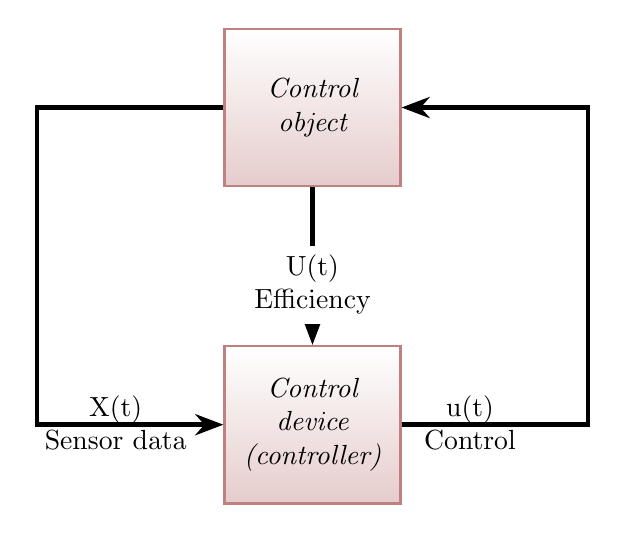
\begin{tikzpicture}[
format/.style={rectangle, thick, minimum size=2cm,draw=red!50!black!50,top color=white,bottom color=red!50!black!20,font=\itshape, node distance=2cm, text width=2cm,align=center }
]
\normalsize{
\node[format]      (maintopic)                              {Control object};
\node[format]      (downsquare)       [below=of maintopic] {Control
device
(controller)};

\path[->, ultra thick, -{Stealth[slant=0]}] (maintopic) edge node {}(downsquare);
\node[node distance=2cm, text width=2cm,align=center,fill=white] at (0, -2.25) {U(t) Efficiency};
\path[->, draw, ultra thick, -{Stealth[slant=0]}] (maintopic) -- +(-3.5,0) |- node[near start] {} (downsquare);
\node[node distance=2cm, text width=1.5cm,align=center] at (2, -4) {u(t) Control};
\path[->, draw, ultra thick, -{Stealth[slant=0]}] (downsquare) -- +(3.5,0) |- node[near start] {} (maintopic);
\node[node distance=2cm, text width=2cm,align=center] at (-2.5, -4) {X(t) \\ Sensor data};}
\end{tikzpicture}
\caption{Reinforcement learning
} \label{fig:M2}
\end{figure}

\begin {figure}[ht]
\includegraphics[width=0.9\columnwidth]{images/pic1.jpg}
\caption{The developed neuro-PID controller, TD means delay
operator}
\label{fig:M3}
\end{figure}

\begin{align*}
u_{k} & =u_{k-1}+\Delta u_{k} \\
\Delta u_{k} & =q_{0} e_{k}+q_{1} e_{k-1}+q_{2} e_{k-2} \\
q_{0} & =\mathbf{K}\left(1+\frac{T_{D}}{T_{0}}\right)  \tag{1}\\
q_{1} & =-\mathbf{K}\left(1+2 \frac{T_{D}}{T_{0}}-\frac{T_{0}}{T_{I}}\right) \\
q_{2} & =\mathbf{K} \frac{T_{D}}{T_{0}}
\end{align*}

Algorithm for operation of \textbf{neuro-PID adjuster} [16]:

\begin {figure}[h]
\includegraphics[width=\columnwidth]{images/pic2.jpg}
\caption{Neuro-adjuster PID}
\label{fig:M4}
\end{figure}
}
     
\end{document}


